\documentclass[bare]{polytech/polytech}
      
\usepackage{lipsum}

\addbibresource{biblio}

\begin{document}

\chapter{Test includepdf}

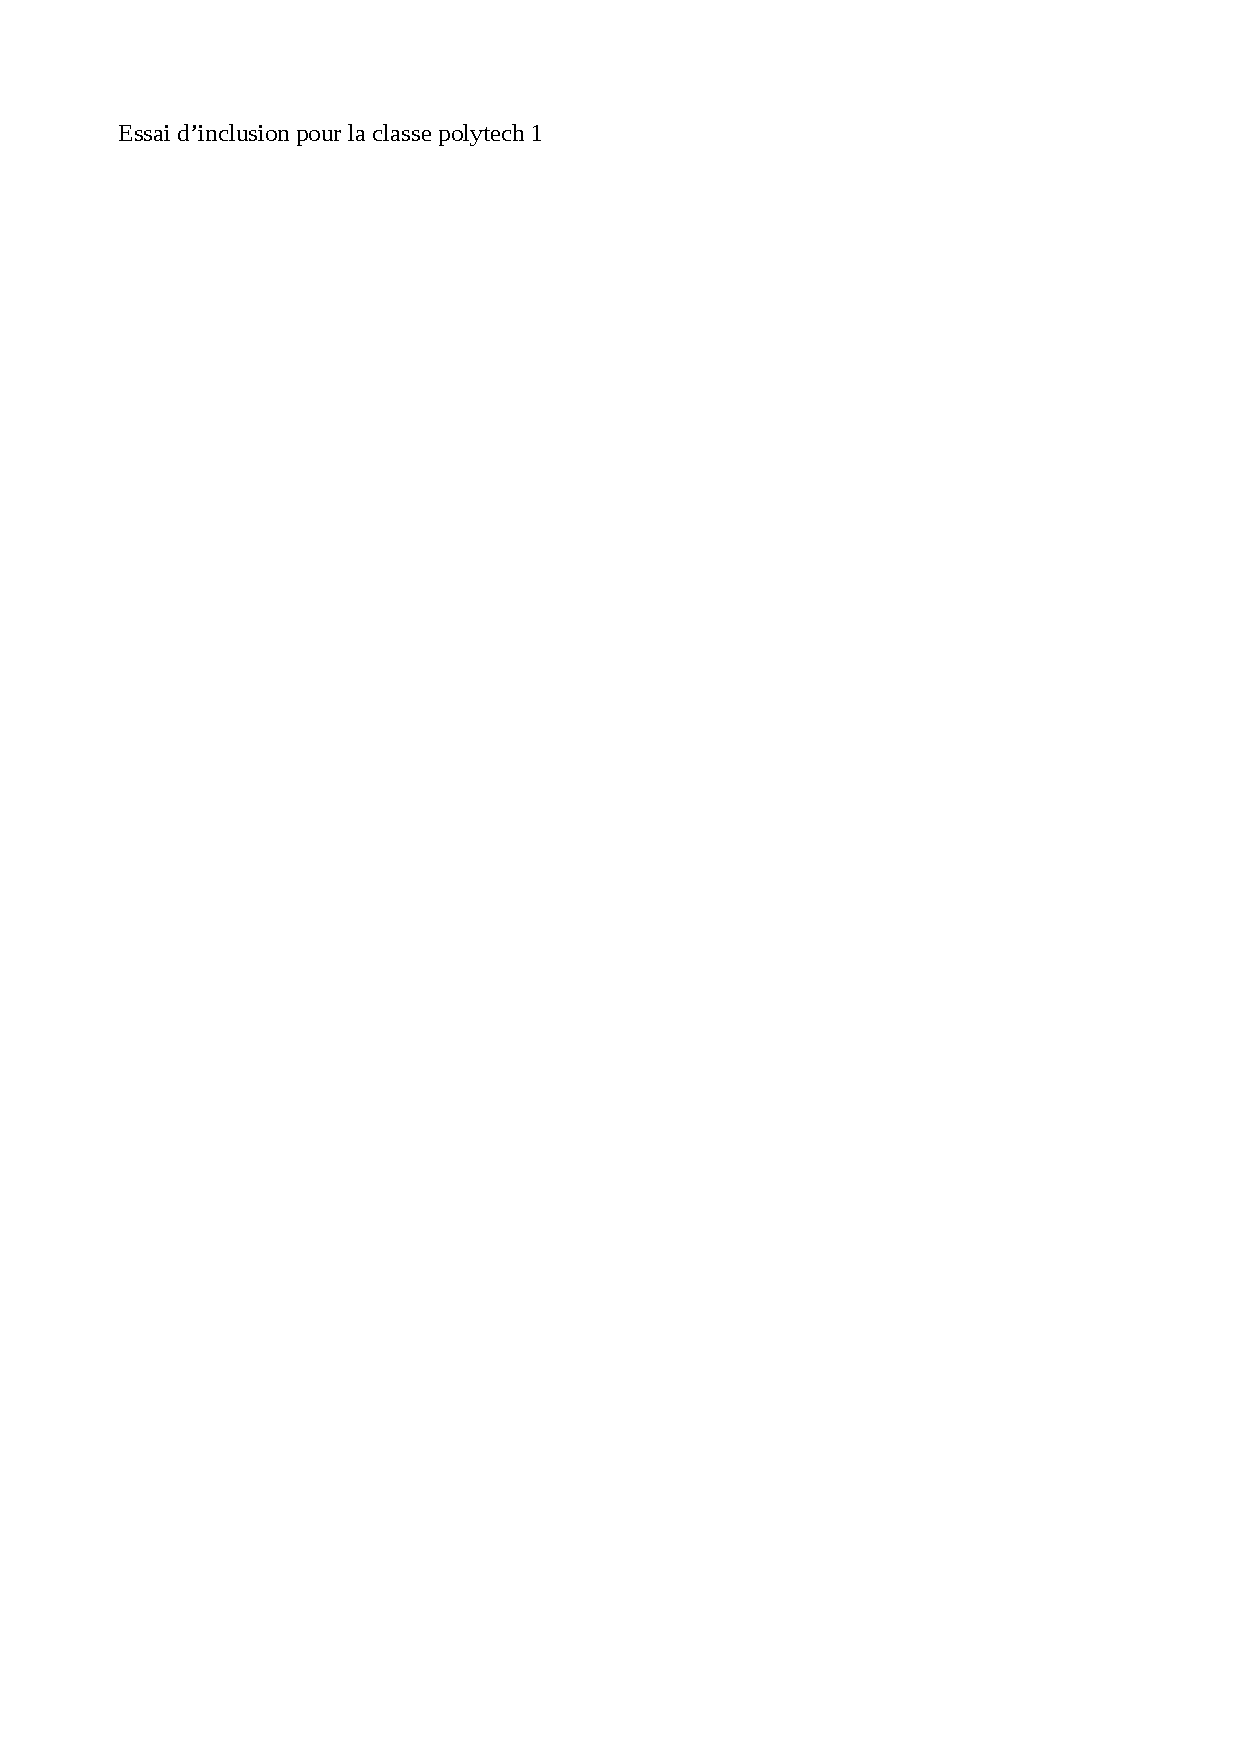
\includepdf[pages=-,templatesize={\textwidth}{\textheight}]{includeme.pdf}            

             
\chapter*[Titre court pour l'entête]{Introduction générale du rapport avec un titre un peu long}

\lipsum[1-5]
\section{Ma section}

\lipsum[1-3]

\subsection{Ma section}

\lipsum[1-3]

\subsubsection{Ma section}

\lipsum[1-3]

\paragraph{Ma section}

\lipsum[1-3]

\subparagraph{Ma section}

\lipsum[1-3]

\section{Une section n'est jamais seule, donc j'en ajoute au moins une autre et le titre peut être long si nécessaire}

\lipsum[1-3]
                       
\section{Le dicton dit \og{}Jamais deux sans trois\fg{}, donc j'en ajoute au moins une autre et le titre peut être long si nécessaire mais il ne faut pas abuser car ça devient moche et peu explicite sinon}

\lipsum[1-3] 

\part{Les premiers trucs dont je vais parler}                

\chapter{Le tout premier truc}   

\lipsum[1]
           
\section{Pour ne pas se casser la tête}

\lipsum[1-6]

\part{essai}
 
\chapter{essai:chap1}
      
\lipsum[1-4]
     
\section{truc}

\chapter*{essai:chap2}
     
\lipsum[1-4]

\section{truc}

  
\chapter{truc}
\lipsum[1-20]         
 
\section{Ma section}
\lipsum[1-5]

\section{Ma section}
\lipsum[1-5]

          
\subsection{Ma section}
\lipsum[1-5]
\subsection{Ma section}
\lipsum[1-5]
\subsubsection{Ma section}
\lipsum[1-5]
\subsubsection{Ma section}
\lipsum[1-5]
\paragraph{Ma section}
\lipsum[1-5]
\paragraph{Ma section}
\lipsum[1-5]
\subparagraph{Ma section}
\lipsum[1-5]
\subparagraph{Ma section}
\lipsum[1-5]
  
\chapter*{Conclusion}

\lipsum[1-2]

\appendix   

\chapter{Ma première annexe}

\lipsum[1-4]

\section{truc}

\lipsum[1-4]
 
\chapter{Ma deuxième annexe}
  

\section{truc}

\lipsum[1-4]

\end{document}


